% !TEX root = ../dsv_script.tex
In \Cref{sec:sampling:sampling_theorem} haben wir eine Theorie entwickelt, welche es uns erlaubt aus einer diskreten Menge von Abtastpunkten, das ursprüngliche Signal zu rekonstruieren.
Allgemeiner kann man dies auch als ein Interpolationsproblem betrachten, wobei es darum geht, eine Funktion zu finden, deren Werte an bestimmten Punkten vorbestimmt sind.
Das heißt, wir suchen nicht unbedingt eine bestimmte Funktion, sondern eine beliebige, die \q{nur} die sogenannte Interpolationseigenschaft erfüllt.
Eine Möglichkeit, solche eine Funktion zu finden, bietet die \gls{dft}.
%
%
\subsubsection{Theoretische Grundlagen}\label{sec:dftintp:theory}
%
Gegeben sei ein periodisches, analoges Signal $x: \R \rightarrow \C$, mit Periode $T_p = 1/F_0$. 
Wir beobachten dieses Signal auf einem uniformen Raster von Punkten, via $x[n] = x(n T)$ und wollen eine Funktion $y$ herleiten, für welche die Interpolationsbedingung
\begin{equation}\label{eq:dftintp:interpol_cond}
    y(nT) = x[n] = x(nT)
\end{equation}
erfüllt ist. 
Hierzu entwickeln wir das Signal $x$ in seine Fourier-Reihe via
\begin{equation}\label{eq:dftintp:fourier_series}
    x(t) = \Sum{k=-\infty}{+\infty}{
        c[k] \exp(\jmath 2 \pi k t F_0) 
    },
\end{equation}
womit nun \q{nur} noch die Fourierkoeffizienten $c[\cdot]$ zu finden sind.
Nun tasten wir dieses Signal uniform mit Samplerate $F_s = N/T_p = 1/T$ (also passend zur Periodendauer) ab und erhalten die Folge 
\begin{equation}
    x[n] = x(n T) = \Sum{k=-\infty}{+\infty}{
        c[k] \exp(\jmath 2 \pi k n T F_0) 
    } = \Sum{k=-\infty}{+\infty}{
        c[k] \exp\left(\jmath 2 \pi k \frac nN\right) 
    }
    \Text{für}
    n \in \N
\end{equation}
bestehend aus den Samples von $x$ an deren Stellen die Interpolationsbedingung erfüllt sein soll. 
Mit der Periodizität von $\exp(\jmath 2 \pi t)$, siehe \Cref{sec:fourier:disc_period} und \Cref{sec:sampling:disc_sin}, und der Abtastung erhalten wir außerdem noch
\begin{equation}
    x[n] = \Sum{k=0}{N-1}{
        \left[\Sum{\ell=-\infty}{+\infty}{
            c[k - \ell N]
        }\right] \exp\left(\jmath 2 \pi k \frac nN\right) 
    } = \Sum{k=0}{N-1}{
        \tilde{c}[k] \exp\left(\jmath 2 \pi k \frac nN\right) 
    },
\end{equation}
wobei wir 
\begin{equation}\label{eq:dftintp:aliased_ck}
    \tilde{c}[k] = \Sum{\ell=-\infty}{+\infty}{
        c[k - \ell N]
    }
\end{equation}
als Abkürzung benutzt haben. 
Wir nehmen nun aus guten Grund noch an, dass die Funktion $x$ auch bandbegrenzt ist.
Das heißt, ihre Fourier-Transformierte $X : \R \rightarrow \C$ verschwindet außerhalb eines gewissen Bandes, also
\begin{equation}
    X(F) = \Int{-\infty}{+\infty}{x(t) \exp(-\jmath 2 \pi F t )}{t} = 0 \Text{für} \Abs{F} > B.
\end{equation}
Außerdem wissen wir, dass die Fourier-Transformation $X$ und die Folge $c[k]$ verknüpft sind via 
\begin{equation}
    c[k] = \frac{1}{T_p} X(k F_0),
\end{equation}
was impliziert, dass die Folge $c[k]$ ab einem gewissen $k > K_0$ verschwindet.
Es gilt also
\begin{equation}
    c[k] = 0 \Text{für} \Abs{k} > \left\lceil \frac{B}{F_0} \right\rceil.
\end{equation}
Das heißt, dass wir nun $F_s = N/T_p$ so groß wählen müssen, dass sich in \eqref{eq:dftintp:aliased_ck} kein Aliasing für $\tilde{c}[k]$ ergeben kann.
Es muss also gelten
\begin{equation}
    N > \lceil B/F_0 \rceil \Text{bzw.} F_s > \lceil B/(F_0 T_p) \rceil.
\end{equation}
Es folgt dann, dass $c[k] = X[k]$, wobei $X[k]$ die \gls{dft} der Folge $x[n]$ darstellt. 
Das heißt, dass wir die Fourier-Koeffizienten der kontinuierlichen Funktion $x$ durch die \gls{dft} der Abtastwerte $x[n]$ bestimmen können. 
Mit \eqref{eq:dftintp:fourier_series} können wir also die Folge $x[n]$ interpolieren, indem wir
\begin{equation}\label{eq:dftintp:dft_interpolation}
    y(t) = \frac{1}{T_p}\Sum{k=-\frac{B}{F_0}}{+\frac{B}{F_0}}{
        X[k] \exp(\jmath 2 \pi k t F_0) 
    }
\end{equation}
schreiben. 
Dieses $y$ erfüllt die Interpolationsbedingung \eqref{eq:dftintp:interpol_cond}, weil wegen der Bandbegrenzung von $x$ und der Periodizität sogar $y(t) = x(t)$ für alle $t$ gilt.

Man beachte hier, dass nun aus der Folge von diskreten Werten $x[n]$ eine analytische Formel in Form einer \emph{endlichen} Summation entstanden ist. 
Unter der Annahme der Bandlimitierung von $x$ ist diese Interpolation \emph{exakt} und kann effizient implementiert werden, durch die Vorberechnung der Folge $X[k]$ durch die \gls{fft}~\cite{FFTW05} der Folge $x[n]$. 
Eine Anwendung der hier vorgestellten Methode zur Interpolation wird in \cref{sec:eadf} aufgezeigt.
%
%
%
%
\FloatBarrier
\subsubsection{Interpolation von Antennen-Richtcharakteristiken}\label{sec:eadf}
%
\paragraph{Motivation}
%
%
Mit jeder Erschließung von neuen Frequenzbereichen für die Kommunikation ist es von Interesse das Ausbreitungsverhalten der elektro-magnetischen Wellen für verschiedene Umgebungen zu charakterisieren, beispielsweise innerstädtisch, auf der Autobahn, etc.
Zwar können solche Umgebungen auch computerbasiert simuliert werden, doch für eine empirisch abgeleitete Statistik solcher sogenannter Kanalmodelle~\cite{delgaldo2007phd} sind repräsentative Messungen unerlässlich. 
Diese Charakteristiken werden genutzt, um in realistischen Szenarien Kanalkapazitäten, Datenraten und dergleichen zu bestimmen. 
Schlussendlich fließen solche Statistiken dann in neue Mobilfunkstandards ein, indem jene Statistiken zur Quantifizierung der Performance von beispielsweise Endgeräten herangezogen werden.

\begin{figure}
    \centering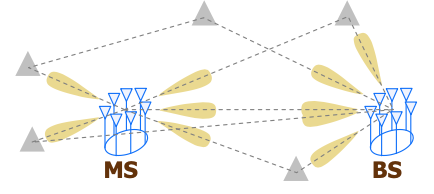
\includegraphics[width=0.6\textwidth]{img/eadf/sounding.png}
    \caption{Schematische Darstellung einer \acrshort{mimo} Kanalmessung. Grafik aus~\cite{richter_estimation_2005}.}\label{fig:eadf:sounding}
\end{figure}

Das FG EMS hat sich deshalb unter anderem auf solche Messungen und deren Auswertung, das sog. Channel Sounding~\cite{thomae2005multidim_hrpe}, spezialisiert. Hierbei kommen meist breitbandige \gls{mimo} Messsysteme zum Einsatz, die den Funkkanal in Frequenz, Raum und Zeit kohärent vermessen können, wie in \Cref{fig:eadf:sounding} dargestellt. Anschließend nutzt man spezielle Signalverarbeitungstechniken~\cite{semper2023wideband_channel_sounding}, die einerseits unter gewissen physikalischen Annahmen das Ausbreitungsverhalten aus den gemessenen Daten ableiten können, und andererseits gleichzeitig den Einfluss des Messsystems so weit wie möglich aus den geschätzten Kanalstatistiken entfernen. Schließlich ist man an der Realität außerhalb des Messaufbaus interessiert. 

Natürlich sind hierzu vor der Messung präzise Kalibriermessungen des Systems notwendig.
Wir wollen uns im folgenden auf die Wirkung der benutzten Antennenarrays konzentrieren, da diese -- wie wir sehen werden -- eine gewisse Sonderbehandlung benötigen.
Zunächst stellt man bei der Konzipierung und Benutzung des Messsystems sicher, dass es sich um ein \gls{lti} System handelt.
Betrachtet man nun das Verhalten des Systems im Frequenzbereich für ein einzelnes Paar von Sende- und Empfangsantenne, dann gilt demnach zunächst
\begin{equation}
    Y(f) = G_{\rx}(f) \cdot H(f) \cdot G_{\tx}(f) \cdot X(f).
\end{equation}
Hierbei steht $X$ für die Anregung des Systems durch ein eingegebenes Signal, $G_{\tx/\rx}$ für die Transferfunktion der Sender- bzw. Empfängerhardware, und $H$ für die Transferfunktion des Funkkanals, der demnach auch als ein \gls{lti} System modelliert wird.
Es stellt sich aber heraus, dass jede Antenne eine \emph{winkelabhängige} Richtcharakteristik besitzt.
Das heißt, dass die Systemantworten $G_{\tx/\rx}$ davon abhängig sind, in welche Richtungen sich die Wellen vom Sender $\tx$ ausbreiten und aus welchen Richtungen, sie am Empfänger $\rx$ eintreffen. 

Um dies korrekt zu modellieren, muss man sich also zunächst auf einzelne sog. \emph{Ausbreitungspfade} konzentrieren.
Das heißt wir nehmen an, dass eine ebene Welle sich in die normierte Richtung $\Omega_{\tx}$ ausbreitet und nach ihrem Weg durch den Funkkanal am Empfänger aus normierter Richtung $\Omega_{\rx}$ eintrifft. 
Folglich ergibt sich für dieses Verhalten
\begin{equation}\label{eq:eadf:single_path}
    Y(f, \Omega_{\tx}, \Omega_{\rx}) = 
        G_{\rx}(f) \cdot a_{\rx}(f, \Omega_{\rx})
        \cdot H(f, \Omega_{\tx}, \Omega_{\rx}) 
        \cdot a_{\tx}(f, \Omega_{\tx}) \cdot G_{\tx}(f)
        \cdot X(f),
\end{equation}
%
wobei $a_{\tx/\rx}$ für die richtungs- und frequenzabhängige Antwort der Sende- und Empfangsantenne stehen.
In diesem Fall bezeichnet also $H(f, \Omega_{\tx}, \Omega_{\rx})$ die Transferfunktion eines einzelnen Pfades, der den Sender in Richtung $\Omega_{\tx}$ verlässt und am Empfänger aus Richtung $\Omega_{\rx}$ eintrifft.
Das heißt, wir haben in diesem Fall das Verhalten der Antennen vom Rest des Systems isoliert. 

Die Transferfunktion für die gesamte Messung wird dann als Summe der Transferfunktionen solcher ebenen Wellen modelliert, also via
\begin{equation}
    Y(f) = \Sum{s = 1}{S}{
        Y(f, \Omega_{\tx,s}, \Omega_{\rx,s})
    },
\end{equation}
was sich dadurch rechtfertigt, dass die Transferfunktion des Kanals sich aus der Lösung einer partiellen Differentialgleichung ergibt, deren Lösungsraum lineare Struktur hat.
Es zeigt sich aus \eqref{eq:eadf:single_path}, dass wir eine möglichst präzise Formulierung für $a_{\tx/\rx}$ benötigen, um die Transferfunktion des Kanals $H$ korrekt bestimmen zu können.
%
%
%
\paragraph{Messvorgang}
%
%
Es ist also unsere Aufgabe für eine gegebene Antenne ein parametrisches Modell $a: [0, \pi] \times [0, 2\pi] \rightarrow \C$ der Form $a(\varphi, \vartheta) \in \C$, also in Betrag und Phase, herzuleiten.
Aus Gründen der Einfachheit und der Physik vernachlässigen wir die Frequenzabhängigkeit der Antenne und konzentrieren uns auf ihr Verhalten für die Anregung mit einer einzelnen Frequenz.
Auch die Polarisation von ebenen Wellen und das davon abhängige Verhalten einer Antenne vernachlässigen wir hier.
Wir konzentrieren uns also auf die \emph{Winkelabhängigkeit} der Antennenantwort.

Wie oben motiviert benötigen wir eine kontinuierliche Beschreibung der Antennenantwort.
Doch diese ist uns wegen endlichem Speicherplatz auf Festplatten und angepeilter endlicher Messzeit nicht direkt zugänglich.
Man weiß jedoch, dass es einen Zusammenhang zwischen der elektrischen Größe einer Antenne und deren winkelabhängigen Verhalten gibt~\cite[Kapitel~4]{delgaldo2007phd}.
Das heißt, man kann zeigen, dass die Funktion $a$ \emph{bandbegrenzt} ist, beziehungsweise sich sehr gut durch eine bandbegrenzte Funktion \emph{approximieren} lässt.
Weiterhin ist durch die Stetigkeit der Physik jede Antennencharakteristik periodisch.
\emph{$\ast$Fourier-Reihen-Sound intensifies$\ast$}

\begin{figure}[t]
    \centering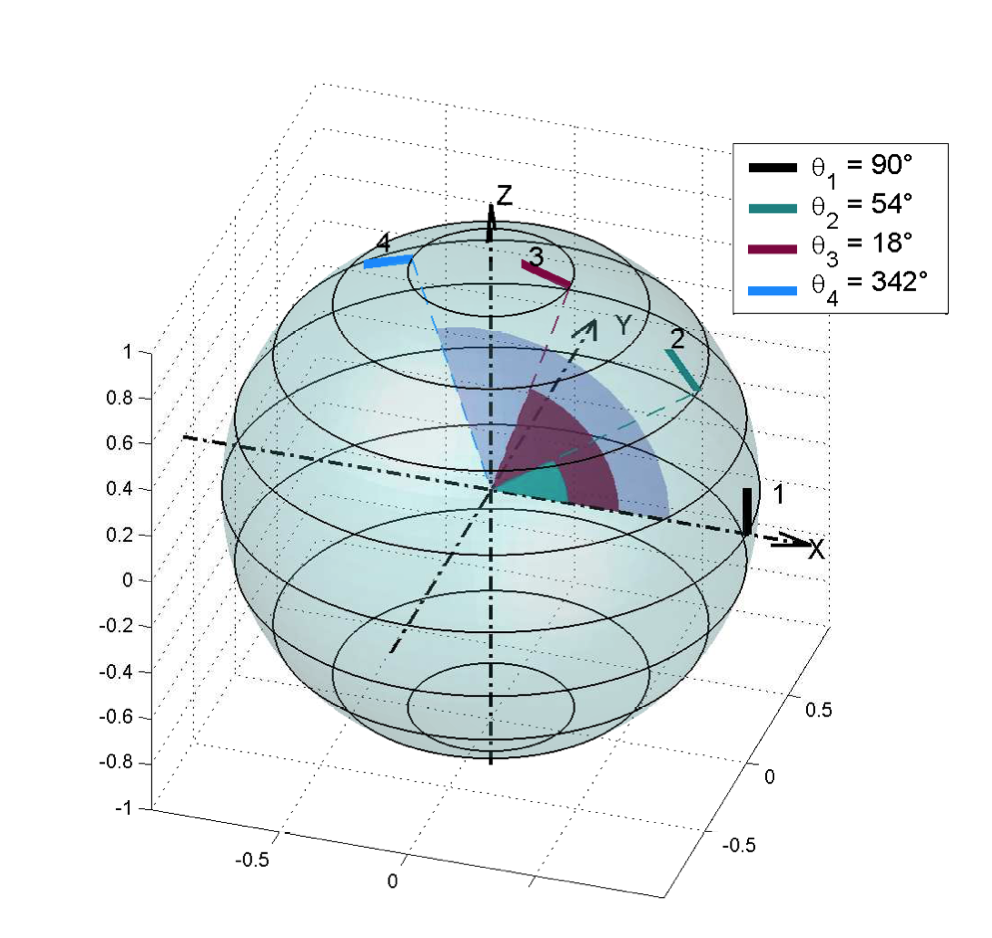
\includegraphics[width=0.49\textwidth]{img/eadf/measure.png}
    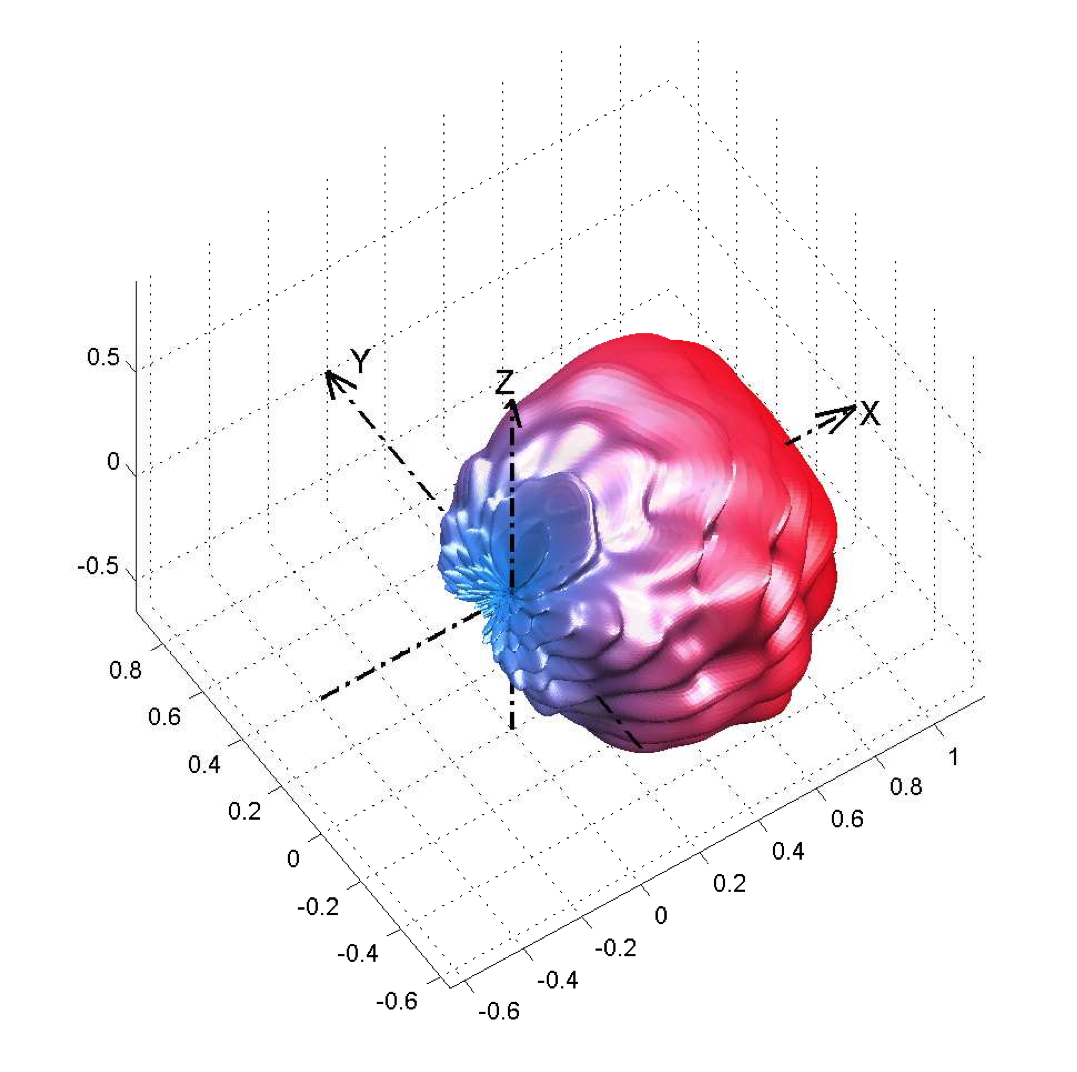
\includegraphics[width=0.49\textwidth]{img/eadf/3d_bp.png}
    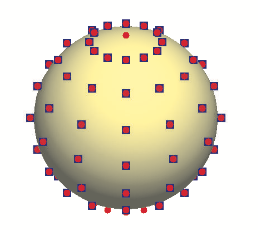
\includegraphics[width=0.3\textwidth]{img/eadf/bp_sampling.png}
    \caption{Links Oben: Darstellung der Messpositionen für eine Antenne, oder eine Antennenstruktur, welche sich im Ursprung des abgebildeten Koordinatensystems befindet. Rechts Oben: Darstellung der winkelabhängigen Amplitude eines einzelnen Patch-Elements. Unten: Messpunkte für die Abtastung der Funktion $a$. Grafiken aus \cite{landmann2004EADF,delgaldo2007phd}.}\label{fig:eadf:meas}
\end{figure}

Das heißt weiterhin, dass es uns möglich ist, die Antenne an diskreten Stellen abzutasten, sodass wir mit der Annahme der Bandbegrenzung und der Aussage des Nyquist-Theorems ein Modell ableiten können, welches die Antenne vollständig charakterisiert.
In diesem Sinne geht es darum die kontinuierliche Antennenantwort $a$ zu ``digitalisieren''.
Die ``Abtastung'' erfolgt demnach im Winkelbereich. Der zugehörige ``Frequenzbereich'' ist entsprechend der \emph{räumliche Frequenzbereich}.
\Cref{fig:eadf:meas} zeigt einerseits schematisch den Messaufbau, das genutzte Koordinatensystem und beispielhaft die 3D-Darstellung einer Antennenantwort eines einzelnen Patch-Elements.

Die Messung selbst erfolgt in einer echofreien Messkammer, in welcher es möglich ist, die \gls{aut} beliebig relativ zu einer bereits kalibrierten Referenzantenne zu verdrehen, sodass ein Abtastraster, wie in \Cref{fig:eadf:meas} unten gezeigt, entsteht.
Pro Ausrichtung wird die \gls{aut} für gewöhnlich für mehrere Frequenzen, zwei orthogonale Polarisationen und alle ihre Elemente vermessen, bevor die nächste Ausrichtung angefahren wird.
Wie erwähnt konzentrieren wir uns auf eine einzelne Frequenz, ein einzelnes Element und eine seiner Polarisationen.
In \Cref{fig:eadf:anechoic} sieht man den Messaufbau, der von unserem FG benutzt wurde, um ein Antennenarray mit 32 Elementen zu vermessen.

\begin{figure}[t]
    \centering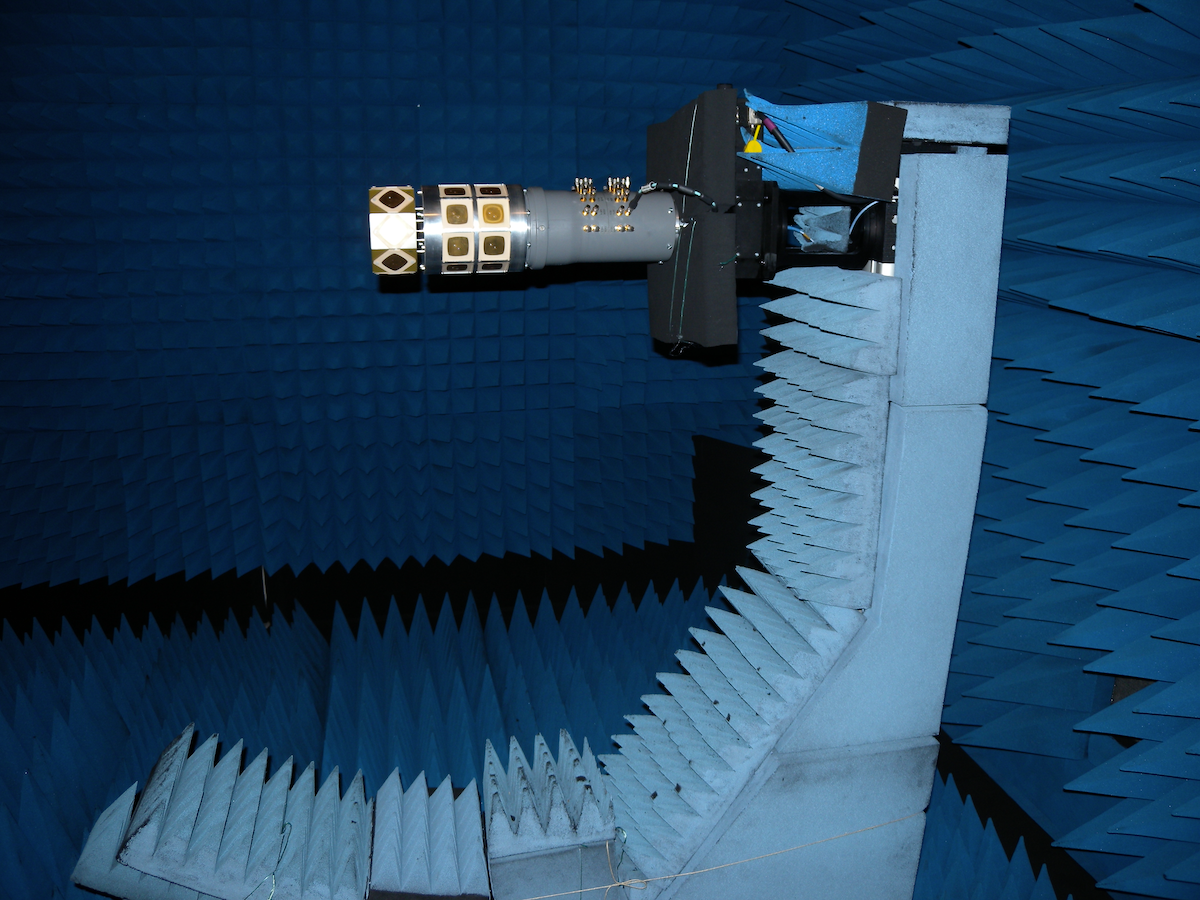
\includegraphics[width=0.49\textwidth]{img/eadf/anechoic1.png}
    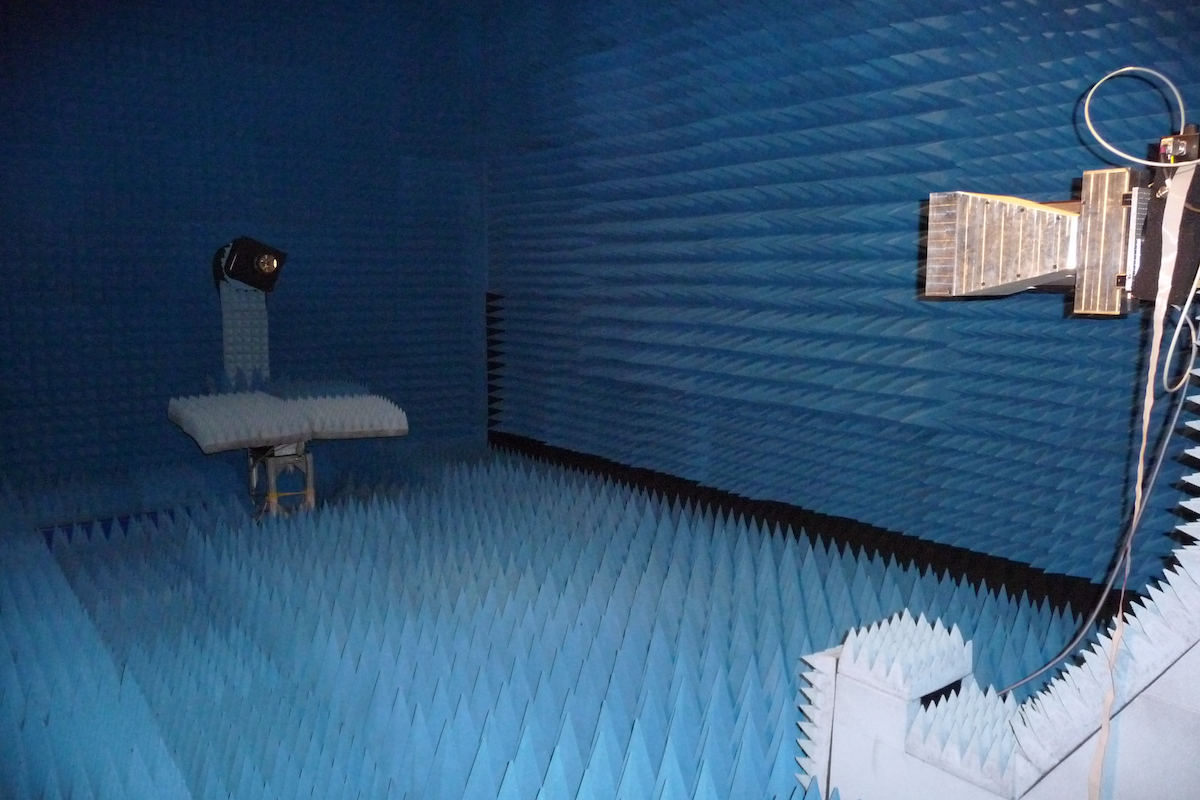
\includegraphics[width=0.49\textwidth]{img/eadf/anechoic2.png}
    \caption{Messaufbau zur Kalibrierung eines Antennenarrays. Links: Drehteller für die Positionierung der \gls{aut}. Rechts: Weiterer Blickwinkel mit Referenzantenne.}\label{fig:eadf:anechoic}.
\end{figure}

Für ein einzelnes Antennenelement beobachten wir also die Funktion $a$ auf einem Gitter, das aus allen Kombinationen der Punkte 
\[
    \varphi_0, \dots, \varphi_{N_\varphi}, \varphi_i = \frac{i \pi}{N_\varphi}
    \Text{und}
    \vartheta_0, \dots, \vartheta_{N_\vartheta-1}, \vartheta_j = \frac{j 2 \pi}{N_\vartheta}
\]
besteht.
Wir erhalten also ein zweidimensionales Array $a[i,j] \in \C^{N_\varphi \times N_\vartheta - 1}$, welches wir noch durch einen Trick geeignet periodifizieren müssen, wie in \Cref{fig:eadf:bp_aperture} links dargestellt.
Diese Abtastwerte entspringen also einer zweidimensionalen bandbegrenzten, periodischen Funktion.
Aufgabe ist es nun aus diesen Werten eine geeignete Interpolante herzuleiten, die sich diese beiden Eigenschaften zunutze macht.
%
%
%
%
%
%
\paragraph{Ableitung der EADF}
%
%
Wir wollen nun \eqref{eq:dftintp:dft_interpolation} aus \Cref{sec:dftintp} benutzen und auf zwei Dimensionen erweitern.
Wir folgen damit effektiv~\cite{landmann2004EADF}.
Außerdem ändern wir das Argument der Funktion $x$ und deren Namen zu der oben eingeführten Schreibweise $a : [0, 2 \pi] \times [0, 2 \pi] \rightarrow \C$ mit Werten $a(\varphi, \vartheta)$. 
In unserem Fall der Interpolation von Antennenantworten wissen wir, dass $a$ in \emph{beiden} Argumenten $2\pi$-periodisch ist.

\begin{figure}[t]
    \centering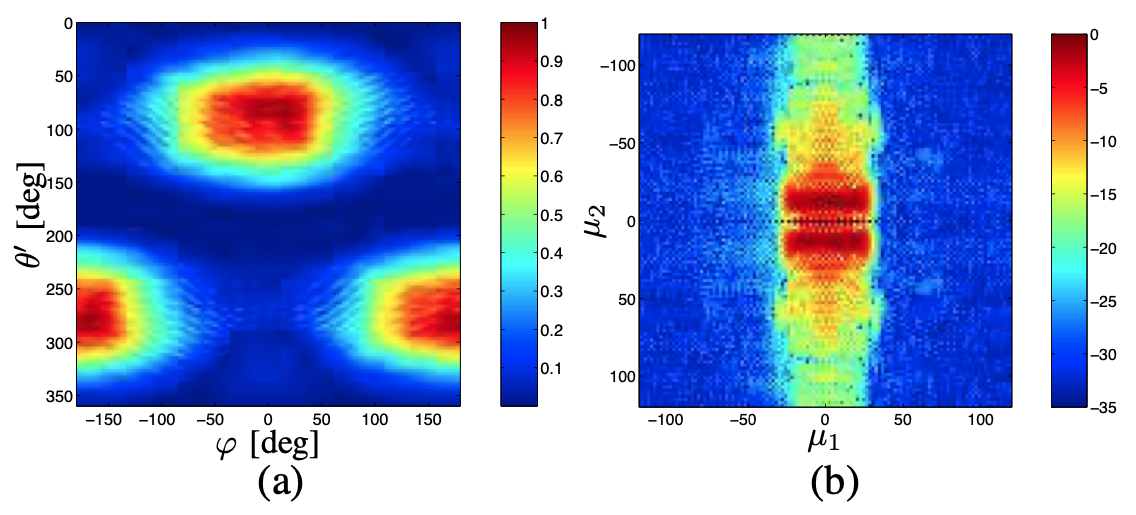
\includegraphics[width=0.75\textwidth]{img/eadf/bp_aperture.png}
    \caption{Links: Periodifizertes 2D Array $a[n_\varphi, n_\vartheta]$ der gemessenen Amplituden eines einzelnen Patch-Elements. Rechts: Der Betrag der zugehörigen \gls{eadf}, wobei hier $\mu_1 = k_\varphi$ und $\mu_2 = k_\vartheta$. Grafik aus~\cite{landmann2004EADF}}\label{fig:eadf:bp_aperture}
\end{figure}

Die Bandlimitierung von $a$ lässt sich formulieren, indem man fordert, dass die Bedingungen
\begin{align}
    A_{\varphi}(F_\varphi, \vartheta) 
    &= \Int{-\infty}{+\infty}{
        a(\varphi, \vartheta) \exp(-\jmath 2 \pi F_\varphi \varphi)
    }{\varphi} = 0 
    \fuer F_\varphi > B_\varphi \Text{und alle} \vartheta \in [0, 2 \pi] \Text{und} \\
    A_{\vartheta}(\varphi, F_\vartheta) 
    &= \Int{-\infty}{+\infty}{
        a(\varphi, \vartheta) \exp(-\jmath 2 \pi F_\vartheta \vartheta)
    }{\varphi} = 0 
    \fuer F_\vartheta > B_\vartheta \Text{und alle} \varphi \in [0, 2 \pi]
\end{align}
erfüllt sein müssen.
Nun lassen sich alle obigen Argumente in \Cref{sec:dftintp:theory} \q{schnittweise} auf eine abgetastete Version von $a$ in der Form $a[n_\varphi, n_\vartheta]$ anwenden. 
Das heißt, wir landen schlussendlich bei einer Interpolations-Formel
\begin{equation}\label{eq:eadf:2d_dft_interpolation}
    a(\varphi, \vartheta) = \Sum{k_\varphi=-\frac{B_\varphi}{F_\varphi}}{+\frac{B_\varphi}{F_\varphi}}{
        \Sum{k_\vartheta=-\frac{B_\vartheta}{F_\vartheta}}{+\frac{B_\vartheta}{F_\vartheta}}{
            A[k_\varphi, k_\vartheta] 
            \cdot \exp(\jmath 2 \pi k_\varphi \varphi F_\varphi)
            \cdot \exp(\jmath 2 \pi k_\vartheta \vartheta F_\vartheta)
        }
    },
\end{equation}
welche eine absolut analoge (nicht als Gegenteil zu digitale) $2D$-Version zu \eqref{eq:dftintp:dft_interpolation} darstellt.
Auch in diesem Fall, können wir das $2D$-Array $A[k_\varphi, k_\vartheta]$ durch eine $2D$-\gls{dft}, bzw. der \gls{fft}~\cite{FFTW05}, von den uniformen Samples $a[n_\varphi, n_\vartheta]$ der Funktion $a$ effizient vorberechnen.

Um einen möglichst effizienten Algorithmus für die Auswertung der Interpolante zu erhalten, sollte man \eqref{eq:eadf:2d_dft_interpolation} geeignet umschreiben.
Moderne Rechenarchitekturen und Scientific-Computing-Libraries sind auf schnelle Matrix-Vektor-Produkte optimiert.
Nehmen wir an, wir wollen \eqref{eq:eadf:2d_dft_interpolation} für mehrere Winkelpaare $(\varphi_1, \vartheta_1), \dots, (\varphi_L, \vartheta_L)$ auswerten.
Dann berechnen wir zunächst zwei $2D$ Arrays
\begin{align}
    D_\varphi &= [\exp(\jmath 2 \pi k_\varphi \varphi F_\varphi)]_{\ell = 1, k_\varphi=-\frac{B_\varphi}{F_\varphi}} \in \C^{L \times 2 \frac{B_\varphi}{F_\varphi} + 1} \Text{und}\\
    D_\vartheta &= [\exp(\jmath 2 \pi k_\vartheta \vartheta F_\vartheta)]_{\ell = 1, k_\vartheta=-\frac{B_\vartheta}{F_\vartheta}} \in \C^{L \times 2 \frac{B_\vartheta}{F_\vartheta} + 1}, 
\end{align}
was uns erlaubt \eqref{eq:eadf:2d_dft_interpolation} in das folgende Vektor-Matrix-Vektor-Produkt
\begin{equation}\label{eq:eadf:fast_2d_dft}
    a(\varphi_\ell, \vartheta_\ell) = 
        D_\varphi[\ell, :] \cdot A[:,:] \cdot D_\vartheta[\ell, :]^\trans
\end{equation}
umzuschreiben.
Damit besteht der Interpolations-Algorithmus zunächst aus der Vorberechnung des Arrays $A$, sowie bei Ausführung dann aus der Berechnung von $D_\varphi$ und $D_\vartheta$, sowie der Auswertung von \eqref{eq:eadf:fast_2d_dft}.

Man sieht hier der schön, dass die Laufzeitkomplexität von \eqref{eq:eadf:fast_2d_dft} maßgeblich von der räumlichen Bandbegrenzung der Antennen-Richtcharakteristik beeinflusst wird.
Je höher die Bandbreite, desto höher ist nicht nur der Aufwand bei der Messung, sondern auch bei der Berechnung Interpolation.
Eine alternative Form der Interpolation, welche diese eventuell nachteilige Eigenschaft nicht hat, ist in \Cref{sec:bsplines} dargestellt.
